% Author: Seongjin Lee 
% Hanyang University, Seoul, Korea 
% esos.hanyang.ac.kr 
% 2016-09-11
% note: some slides are adopted from  \url{www.cs.stevens.edu/~jschauma/631A/}
% https://github.com/resourceful/lecture_sysprog/

\documentclass[newPxFont,sthlmFooter,nooffset]{beamer}
\usepackage{kotex}
%\usetheme{sthlm}
\usepackage{../beamer_template/beamerthemesthlm}
\hypersetup{pdfauthor={Seongjin Lee (insight@hanyang.ac.kr)},
            pdfsubject={Lecture Note: System Programming},
            pdfkeywords={Lecture Note, System Programming, class, undergraduate},
            pdfmoddate={D: \pdfdate},
            pdfcreator={Seongjin Lee}}

%\setbeamertemplate{footline}[text line]{%
%    \parbox{\linewidth}{\vspace*{-8pt} \insertsectionhead  \hfill\insertshortauthor\hfill\insertpagenumber}}
%\setbeamertemplate{navigation symbols}{}



\title{System Programming}
\subtitle{Week 3: File I/O}
\author[SJL]{Seongjin Lee}
\institute{\href{mailto:insight@hanyang.ac.kr}{insight@hanyang.ac.kr}\\\url{http://esos.hanyang.ac.kr}\\Esos Lab. Hanyang University}
\date{2016-09-21} 

\begin{document}



\frame[plain]{\titlepage} 

\frame{\frametitle{Table of contents}\tableofcontents} 


%---------------------------------------------------------
\section{File I/Os} 

\begin{frame}[t]{File Descriptors}
\begin{enumerate}[ ]
\item <1-> A {\em file descriptor} (or {\em file handle}) is a small, non-negative integer which identifies a file to the kernel.
\item <2-> Traditionally, \texttt{stdin}, \texttt{stdout} and \texttt{stderr} are 0, 1 and 2 respectively.
\item <3-> \hfill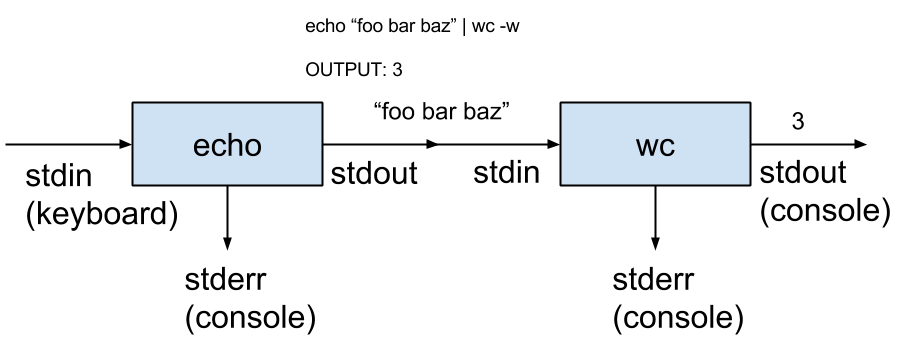
\includegraphics[width=0.7\linewidth]{./figure/stream-pipe.png}\hfill~
\item <4-> Relying on ``magic numbers'' is BAD.  Use \texttt{STDIN\_FILENO}, \texttt{STDOUT\_FILENO} and \texttt{STDERR\_FILENO} defined in <unistd.h> or \texttt{stdin}, \texttt{stdout}, and \texttt{stderr} defined in <stdio.h>.

\end{enumerate}
\end{frame}


\begin{frame}[t]{How many files can you open? (./codes/fdcount.c)}
\lstinputlisting[firstline=17,lineskip=-5pt]{./codes/fdcount.c}

How to compile \\
\texttt{\$ cd codes; cc -Wall -g -o fdcount fdcount.c}

\end{frame}


\subsection{Standard I/O}
\begin{frame}[t]{Basic File I/Os}
There are five fundamental \textsc{Unix} file I/O related functions: 
\begin{itemize}
	\item \texttt{open(2)}
	\item \texttt{close(2)}
	\item \texttt{lseek(2)}
	\item \texttt{read(2)}
	\item \texttt{write(2)}
\end{itemize}
\end{frame}

\begin{frame}[containsverbatim,t]{open(2)}

\begin{lstlisting}[frame=single,numbers=none, xrightmargin=8pt]
#include <fcntl.h>
int open(const char *path, int oflag, ... /* mode_t mode */ );
int openat(int fd, const char *path, int oflag, ... /* mode_t mode */ );
\end{lstlisting}
Both return: file descriptor if OK, −1 on error
\bigskip

The \textit{path} parameter is the name of the file to open or create.
\bigskip

Options are specified by the \textit{oflag}
\end{frame}

\begin{frame}[t]{Options are}
\begin{columns}[t]
\begin{column}{0.30\linewidth}
\small \textit{oflag} must be one (and only one) of:
\footnotesize
\begin{itemize}
	\item \texttt{O\_RDONLY}\\ -- Open for reading only
	\item \texttt{O\_WRONLY}\\ -- Open for writing only
	\item \texttt{O\_RDWR}\\ -- Open for reading and writing
\end{itemize}
\end{column}
\begin{column}{0.70\linewidth}
\small and may be OR'd with any of these:
\footnotesize
\begin{itemize}
	\item \texttt{O\_APPEND} -- Append to end of file for each write
	\item \texttt{O\_CREAT} -- Create the file if it doesn't exist. Requires
		{\em mode} argument
	\item \texttt{O\_EXCL} -- Generate error if \texttt{O\_CREAT} and file
		already exists. (atomic)
	\item \texttt{O\_TRUNC} -- If file exists and successfully open in
		\texttt{O\_WRONLY} or \texttt{O\_RDWR}, make length = 0
	\item \texttt{O\_NOCTTY} -- If pathname refers to a terminal device, do
		not allocate the device as a controlling terminal
	\item \texttt{O\_NONBLOCK} -- If pathname refers to a FIFO, block special,
		or char special, set nonblocking mode (open and I/O)
	\item \texttt{O\_SYNC} --  Each write waits for physical I/O to complete
\end{itemize}
\end{column}
\end{columns}
\end{frame}


\begin{frame}[t]{openat(2)}
\texttt{openat(2)} function is equivalent to the open() function except in the case where the path specifies a relative path in an atomic fashion
\bigskip


\begin{itemize}
	\item \texttt{O\_EXEC} -- Open for execute only
	\item \texttt{O\_SEARCH} -- Open for search only (applies to directories)
	\item \texttt{O\_DIRECTORY} -- If path resolves to a non-directory file, fail and set errno to \texttt{ENOTDIR}.
	\item \texttt{O\_DSYNC} -- Wait for physical I/O for data, except
file attributes
	\item \texttt{O\_RSYNC} -- Block read operations on any pending writes.
	\item \texttt{O\_PATH} -- Obtain a file descriptor purely for fd-level operations. (Linux $>$2.6.36 only)
\end{itemize}

\end{frame}









\section{File Sharing} 

\begin{frame}[t]{File Sharing}
Atomicity of the file fundamental file I/O functions
\bigskip

File sharing
\bigskip

manipulation of file descriptors
\end{frame}


\end{document}
